\ifsvnmulti
 \svnkwsave{$RepoFile: lyapunov/XiongDing.tex $}
 \svnidlong {$HeadURL: svn://zero.physics.gatech.edu/siminos/xiong/blog/Sym.tex $}
 {$LastChangedDate: 2015-05-13 17:26:17 -0400 (Wed, 13 May 2015) $}
 {$LastChangedRevision: 4085 $} {$LastChangedBy: predrag $}
 \svnid{$Id: Sym.tex 4085 2015-05-13 21:26:17Z predrag $}
\fi

\section{Symmetry related}
\label{sect:symm}
\subsection{Bringing infinitesimal variations into the \slice}


% Just like a {\PoincSec},
If the system is invariant under a 1-parameter continuous symmetry,
a \slice\ reduces the dimension of a
system by one. In
order to relate the the full {\statesp}
{\cLvs} to {\cLvs} in the \slice, we need
to relate the \jacobianM\ in full {\statesp}
$\jMps^{t}(x)$ to $\hat{\jMps}^{t}(\sspRed)$ in the \slice. Assume the
group transformation is $\ssp=g(\theta)\sspRed$ (the same with Chaosbook).
    \PC{2014-03-03 you guessed it - we do not like it. It took many deliberations to
    settle on the form in ChaosBook, so why mess with it?}
\Xiong{2014-03-18}{I changed it and a lot of negative sign appears, maybe
there is better way write the blog. {\bf  2014-03-19 Predrag}
I think if you use the transpose, there are no minus signs? And the argument should
also work for \Un{1}\ if you use Hermitian conjugate.
}

\begin{figure}[h]
  \centering
  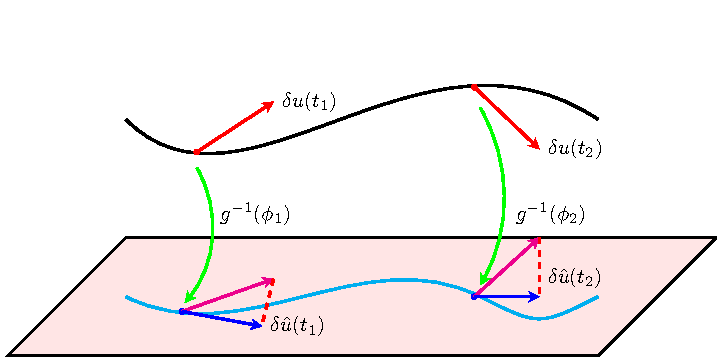
\includegraphics[width=0.7\linewidth]{jacobian_full_slice}
  \caption{The relation between perturbations in
    the full {\statesp} and in the \slice.}
  \label{fig:jacobian_full_slice}
\end{figure}
    \PC{2014-03-19
    please save the source code for \reffig{fig:jacobian_full_slice}
    (and all such figures) in
    \texttt{siminos/figSrc/}
    }
We start from the \slice\ condition
\begin{equation}
\braket{\sspRed}{\sliceTan{}}=0
\label{eq:slicecondition}
\end{equation}
Infinitesimal variation $\delta \sspRed$ at $\sspRed$ in the \slice\
should be confined to the \slice\ too, so we have a constraint
\begin{equation}
\braket{\delta \sspRed}{\sliceTan{}}=0
\,.
\label{eq:constraint_dx}
\end{equation}
(I use Dirac bra-ket notation to avoid the usage of matrix transform
and the repeated indices for dot product, which makes it easier to read);
 On the other hand, from $\ssp=g(\theta)\sspRed$, we have
\[
\delta \sspRed=-\mathbf{T}\sspRed\delta \theta+g(-\theta)\delta\ssp
\,,
\]
where $\mathbf{T}$ is the generator of $g(\theta)$:
$g(\theta)=e^{\mathbf{T}\theta}$. Substitute it into \refeq{eq:constraint_dx},
for \SOn{2}\
we have $\braket{-\mathbf{T}\sspRed\delta \theta+g(-\theta)\delta\ssp}{t'}=0$
 which is
    \PC{2014-03-03 I think it would look prettier if you used bra|ket
    notation $\braket{\cdots}{\cdots}$ throughout. 2014-03-17  edited.}
\begin{equation}
  \label{eq:delta_theta}
  \delta \theta=
      \frac{\braket{\sliceTan{}}{g(-\theta)\delta\ssp}}
            {\braket{\groupTan(\sspRed)}{\sliceTan{}}}
\,.
\end{equation}
Now  $\delta \sspRed$, the infinitesimal variation in the \slice, can be
expressed by  $\delta\ssp$, the variation in the full {\statesp}:
\begin{align*}
  \ket{\delta \sspRed} &=
\frac{\braket{\sliceTan{}}{g(-\theta)\delta\ssp}}
            {\braket{\groupTan(\sspRed)}{\sliceTan{}}}
     \ket{\groupTan(\sspRed)}
    +g(-\theta)\ket{\delta \ssp}\\
\end{align*}
that is,
\beq
\label{eq:variation_full_slice}
\ket{\delta \sspRed} =
    \left(\matId-\frac{\ket{\groupTan(\sspRed)}\bra{\sliceTan{}}}
    {\braket{\groupTan(\sspRed)}{\sliceTan{}}} \right)
    \ket{g(-\theta)\delta \ssp}
    =h(\sspRed)g(-\theta)\ket{\delta \ssp}
\eeq
The physical interpretation of \refeq{eq:variation_full_slice} is manifest:
infinitesimal variation $\delta \ssp$ at $x$ in the full {\statesp} is
 first group transformed to point $\sspRed$ by $g(-\theta)$ and then
projected into the {\slice} by $h(\sspRed)$.
The matrix
\beq
h(\sspRed)=
    \matId-\frac{\ket{\groupTan(\sspRed)}\bra{\sliceTan{}}}
    {\braket{\groupTan(\sspRed)}{\sliceTan{}}}
%\,.
\ee{projFullToSlice}
projects infinitesimal variation in the full {\statesp} into the {\slice}
and it is singular (not full rank) as we can see in a second, so the projection reduces the dimension of the system by one.
Just pointing it out is not enough.  In practice,
we are desired to work in a lower dimensional system after quotienting out
the continuous symmetry and also the
{\slice} condition \refeq{eq:slicecondition}
clearly shows that the components of $\sspRed$ are linear dependent;
however, the left side of \refeq{projFullToSlice} is still expressed in
the full {\statesp}, so decreasing the dimension of all the matrices and
vectors in the {\slice} by one is desired. Before we proceed,
Let's sketch the properties of matrix $h(\sspRed)$ first.
\begin{itemize}
\item $h(\ssp)\ket{t(x)}=0$ : any infinitesimal change along the tangent group
 at $x$
in the full {\statesp} will disappear after projection.
\item $\bra{t'}h(\ssp)=0$ : any vector projected onto the {\slice} will be
perpendicular to the group tangent of the template point as expected. This
property and the above one both prove that matrix $h(\ssp)$ is not full rank.
\item
$
\velRed(\sspRed)=\vel(\sspRed)
-\frac{\braket{\vel(\sspRed)}{\sliceTan{}}}{\braket{\groupTan(\sspRed)}{\sliceTan{}}}
\groupTan(\sspRed)=h(\sspRed)\vel(\sspRed)
\,:
$
\\
The velocity field is transformed by matrix $h(\ssp)$.
\end{itemize}

Now let's reduce the dimension by one. Denote
\[
h(\ssp)=
\begin{bmatrix}
  h_{1} \\
  h_{2} \\
  \vdots \\
  h_{d} \\
\end{bmatrix}
\]
each $h_{i}$ is a row vector and $d$ is the dimension of full {\statesp}.
From the second property of $h(\ssp)$ we know that $h_{i}$ are linear
dependent: $t'_{1}h_{1}+t'_{2}h_{2}+\cdots +t'_{d}h_{d}=0$ here $t'_{i}$ are
components of vector $t'$. Assume $t'_{\xi}\neq 0$ (In Burak's first Fourier mode
{\slice} of \KSe, $\xi=2$ and all other component of $t'$ is zero), then
\[
h_{\xi}=\sum_{i=1,i\neq \xi}^{d}-\frac{t'_{i}}{t'_{\xi}}h_{i}
\]
so $h_{\xi}$ can be eliminated from $h(\ssp)$:
\[
h(\ssp)=
\underbrace{
\begin{bmatrix}
 1 & & & & \\
 & 1 & & & \\
 & & \ddots & & \\
 -\frac{t'_{1}}{t'_{\xi}} & -\frac{t'_{2}}{t'_{\xi}} & & \cdots & -\frac{t'_{d}}{t'_{\xi}} \\
 & & & \ddots  & \\
 & & & & 1 \\
\end{bmatrix}
}_{d\times (d-1)}
\underbrace{
\begin{bmatrix}
  h_{1} \\
  \vdots \\
  h_{\xi-1} \\
  h_{\xi+1} \\
  \vdots \\
  h_{d} \\
\end{bmatrix}
}_{(d-1)\times d}
=P'\hat{h}(x)
\]
The above is the
 \HREF{http://en.wikipedia.org/wiki/Rank_factorization}{rank factorization}
of $h(\ssp)$. Similarly, from the {\slice} condition $\braket{\sspRed}{\sliceTan{}}=0$, we can reduce the dimension of a
point on the {\slice} by one: $\sspRed=P'\sspRed_{p}$, and also an infinitesimal
variation $\delta \sspRed=P'\delta \sspRed_{p}$. Here, $\sspRed_{p}$ and
$\delta \sspRed_{p}$ are both $d-1$ dimensional vectors.
Now relation \refeq{projFullToSlice} can be rewritten as:
\begin{equation}
  \label{eq:projectionReduced}
  \ket{\delta \sspRed_{p}}=\hat{h}(\sspRed)g(-\theta)\ket{\delta \ssp}
\end{equation}
Note that the left side of the above equation $\ket{\delta \sspRed_{p}}$
is a $d-1$ dimensional vector while the right side $\ket{\delta \ssp}$
is a $d$ dimensional vector and the $(d-1)\times d$ matrix $\hat{h}(x)$
is the ``projection'' operator (I give it the name, if you don't like,
just change it. I also suggest replacing the velocity field in the {\slice}
in Chaosbook by $\hat{v}_{p}(\sspRed)=\hat{h}(\sspRed)v(x)$, so
the dimension is one less at the first glance).

Now let's turn to the transformation of {\cLvs}.
For a trajectory from $\ssp(\zeit_1)$ to $\ssp(\zeit_2)$ in the full {\statesp}, the
corresponding transformed trajectory in the \slice\ is from $\sspRed(\zeit_1)$
to $\sspRed(\zeit_2)$.
Infinitesimal variation in the full {\statesp} and in the
{\slice}  will be evolved by
\jacobianM\ in the full {\statesp} and in the {\slice} respectively.
\begin{align*}
 &\hat{\jMps}\delta \sspRed_{p}(t_1)=\delta \sspRed_{p}(t_2) \\
\Rightarrow & \hat{\jMps}\hat{h}(\sspRed(t_1))g(-\theta_1)\delta\ssp(t_1)=
\hat{h}(\sspRed(t_2))g(-\theta_2)\jMps\delta\ssp(t_1)
\end{align*}
so we obtain
\begin{equation}
  \label{eq:relation_jacobian1}
  \hat{\jMps}(\sspRed(\zeit_2),\sspRed(\zeit_1))\hat{h}
(\sspRed(\zeit_1))g(-\theta_{1})=
\hat{h}(\sspRed(\zeit_2))g(-\theta_{2})\jMps(\ssp(\zeit_2),\ssp(\zeit_1))
\,.
\end{equation}
here the $\hat{\jMps}$ is a $(d-1)\times (d-1)$ matrix as we can easily see.
The geometrical meaning of relation \refeq{eq:relation_jacobian1} is obvious
in \reffig{fig:jacobian_full_slice}. On the left side the
infinitesimal variation $\delta \ssp(\zeit_1)$ at $\ssp(\zeit_1)$ is rotated into
$\sspRed(\zeit_1)$, and then projected into the \slice, after which it is
evolved by $\hat{\jMps}$ to $\sspRed(\zeit_2)$. On the right side the
infinitesimal variation $\delta \ssp(\zeit_1)$ at $\ssp(\zeit_1)$ is evolved
first to $\ssp(\zeit_2)$
by $\jMps$, then rotated to $\sspRed(\zeit_2)$, and finally projected
into the \slice.
(I will redraw the illustration \reffig{fig:jacobian_full_slice} after
we get a final version of the argument.)

As  $\hat{h}(\sspRed)$ is an $(d-1)\times d$ matrix, there does not exist
a unique inverse of $\hat{h}(\sspRed(\zeit_1))$ when we tried to get the
\jacobianM\ in the {\slice} from \refeq{eq:relation_jacobian1}.
I am really confused here because we can definitely get the \jacobianM\
from the reduced system in the {\slice}, so the \jacobianM\ should be uniquely
defined, but here \refeq{eq:relation_jacobian1} is not invertible. It means
that we can transform infinitesimal variation in the full {\statesp} into
the {\slice}, but we cannot do the reverse only relying on the information of
$\delta \sspRed$ since the variance in the direction of group tangent
cannot be determined by the variation in the {\slice} $\delta \sspRed$.
Information is lost ? no, $\delta \theta$ contains the information for back
transformation, but I don't know how to use it.

However, for physically interesting invariant orbits (\eqva, \reqva, \po s and \rpo s) , we can
get the relation between
{\cLvs} in the full {\statesp} and in the {\slice}.
For periodic orbits, because $x(0)=x(T_{p})$, we have
$\sspRed(\zeit_1)=\sspRed(\zeit_2)$ and $\theta_{1}=\theta_{2}$, namely
$\hat{h}(\sspRed(\zeit_1))g(-\theta_{1})=
\hat{h}(\sspRed(\zeit_2))g(-\theta_{2})$ in \refeq{eq:relation_jacobian1}.
So, the {\cLvs} are transformed by matrix
$\hat{h}(\sspRed(\zeit))g(-\theta)$. For relative periodic orbits,
$x_{p}(0)=g_{p}x_{p}(T_{p})$, also we have
$\sspRed(\zeit_1)=\sspRed(\zeit_2)$ and $g(-\theta_{1})g_{p}=g(-\theta_{2})$.
Relation in \eqref{eq:relation_jacobian1} becomes
$\hat{\jMps}(\sspRed(\zeit_2),\sspRed(\zeit_1))\hat{h}
(\sspRed(\zeit_1))g(-\theta_{1})
=\hat{h}(\sspRed(\zeit_2))g(-\theta_{1})J_{p}(\ssp(\zeit_2),\ssp(\zeit_1))$,
so covariant vectors are also transformed by
$\hat{h}(\sspRed(\zeit))g(-\theta)$. To sum up, if $e_{i}(x(t))$ is a
covariant vector associated with a (relative) periodic orbit at
point $x(t)$ in the full
state space, then $\hat{h}(\sspRed(\zeit))g(-\theta)e_{i}(x(t))$ is
the corresponding covariant vector at position $\sspRed(\zeit)$ on the
slice, here $x(t)=g(\theta)\sspRed(\zeit)$.

\paragraph{Example: two modes system.}
We follow Chaosbook for the set up of the two modes system and its choice of
parameters. In this example, we only focus on one relative periodic orbit
whose initial condition is $\cycle{1}: (0.4525719, 0.0, 0.0509257,
0.0335428)$. $x'=(1,0,0,0)$ is chosen as the template point the same in
Chaosbook. The multipliers associated with this orbit are
$(-1.481177, -1.066888\cdot 10^{-09}, 0.999414, 0.999913)$. The
neighborhood of this orbit has a week expanding direction and a strong
contracting direction with two marginal directions.

\begin{figure}[h]
  \centering
  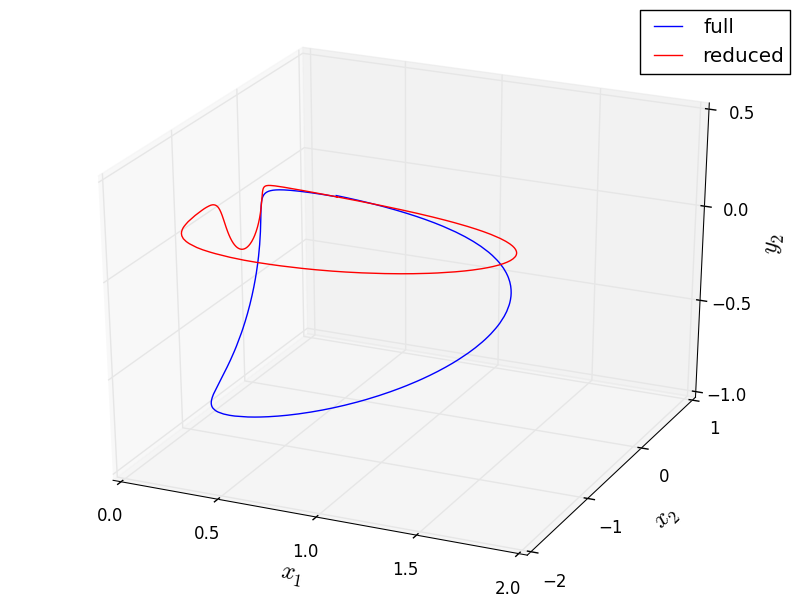
\includegraphics[width=0.8\textwidth]{twomodes_configuration}
  \caption{Configuration of $\cycle{1}$ in the full state space projected
    on to subspace $[x_{1},x_{2},y_{2}]$ (the full one) and on the slice (
    the red one)
  }
  \label{fig:twomodes_configuration}
\end{figure}

\begin{figure}[h]
  \centering
  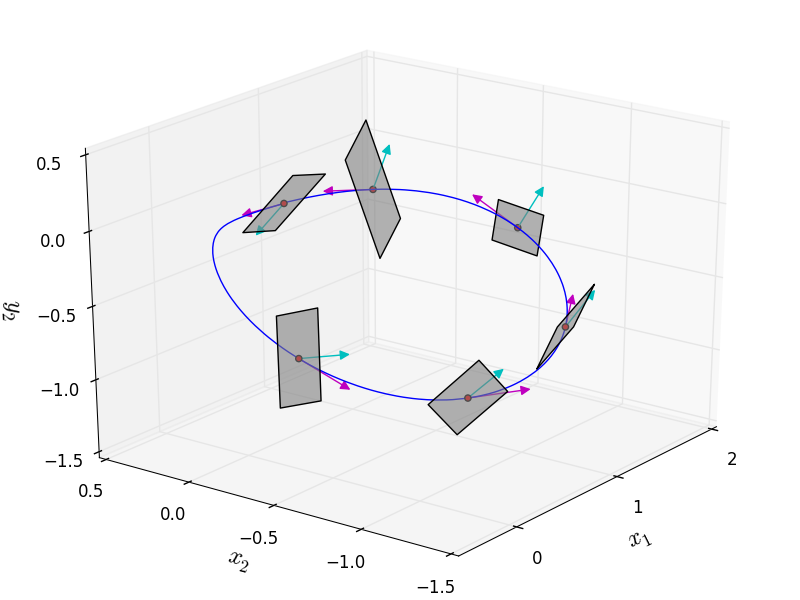
\includegraphics[width=1.0\textwidth]{twomodes_full}
  \caption{The plane spanned by the two marginal eigenvectors of Jacobian
    matrix,
    velocity vector (pink arrow) and group tangent (green arrow)
    in the full state space projected on
    to subspace $[x_{1},x_{2},y_{2}]$.}
  \label{fig:twomodes_full}
\end{figure}

\begin{figure}[h]
  \centering
  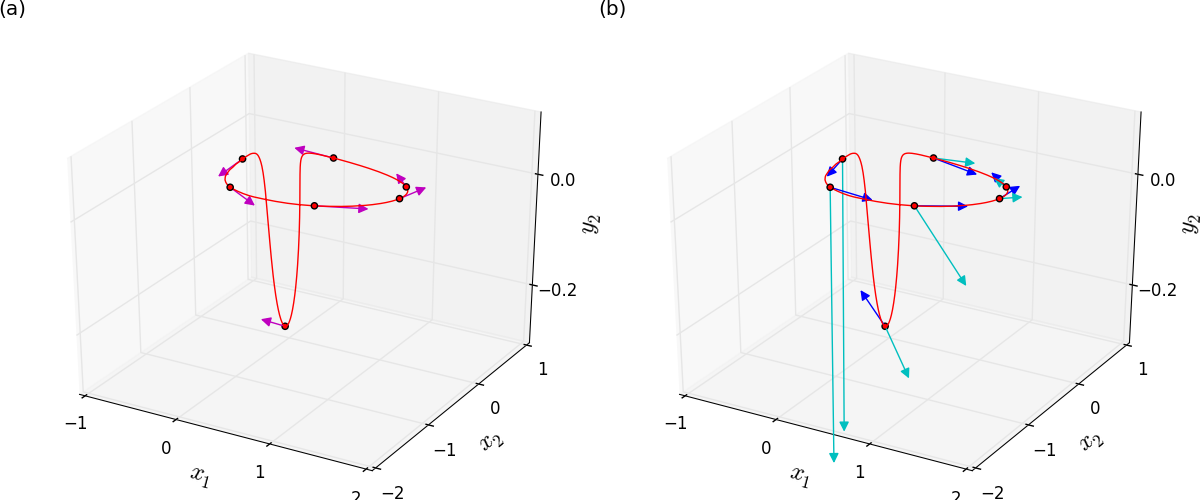
\includegraphics[width=1.0\textwidth]{twomodes_reduced}
  \caption{Covariant vectors in the full state space are projected
    onto the slice. (a) marginal covariant vector (red). (b) expanding
    (blue) and contracting covariant vectors (green) on the slice.
  }
  \label{fig:twomodes_reduced}
\end{figure}

\begin{figure}[h]
  \centering
  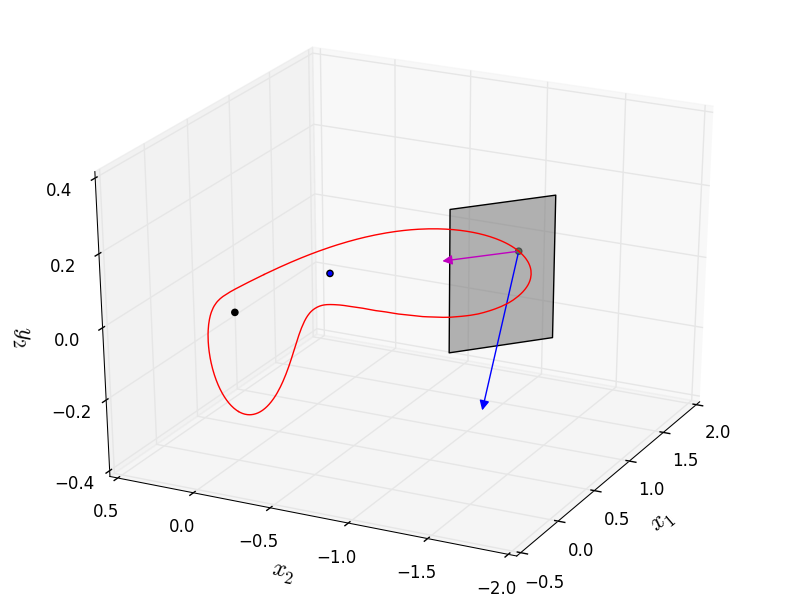
\includegraphics[width=1.0\textwidth]{twomodes_poincare}
  \caption{A vertical poincare section is constructed from fixed point
    (black point) and relative equilibrium
    (blue point) on
    the slice. Covariant vectors on the slice are projected onto the
    Poincare section. The red vector is the expanding one and the blue
    vector is the contracting one. The marginal covariant vector along
    the orbit disappears on the Poincare section.
  }
  \label{fig:twomodes_poincare}
\end{figure}

\begin{figure}[h]
  \centering
  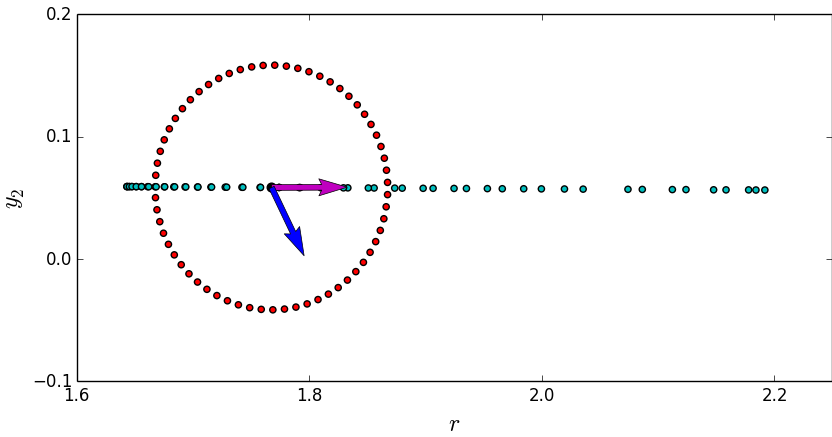
\includegraphics[width=1.0\textwidth]{twomodes_poincare_return}
  \caption{A circularly (radis=0.1) distributed small variances around the intersection
    point of {\PoincSec} and the relative periodic orbit
    \cycle{1} (red dots) are evolved and the first return intersection
    points are recorded (green dots). Red and blue arrows are the expanding
    and contracting
    covariant vectors projected onto the {\PoincSec} respectively.
    Here $r=(\hat{x}_{1}^2+\hat{x}_{2}^2)^{1/2}$
  }
  \label{fig:twomodes_poincare_return}
\end{figure}

\refFig{fig:twomodes_configuration} depicts relative periodic orbit
$\cycle{1}$ in the full state space and on the slice. since both
velocity field $v(x)$ and group tangent $t(x)$ are
marginal covariant vectors along the orbit, these two vectors cannot
be told apart when solving the eigen-function of Jacobian matrix. However,
we can check whether $v(x)$ and $t(x)$ reside on the subspace spanned by
these two eigenvectors of Jacobian matrix. This is the idea of
\reffig{fig:twomodes_full}, and, as we can see, the plane covers $v(x)$ and
$t(x)$ very well. By the way, the two marginal covariant vectors for
pre-periodic orbits in \KS\ system could be told apart. the details are
documented in section \ref{subsect: symkse}.

Now the task is to project these covariant vectors onto the slice, where
the orbit becomes periodic. $t'=(0,-1,0,0)$ and
$t(\sspRed)=(0,-\hat{x}_{1},2\hat{y}_{2},-2\hat{x}_{2})$, so
\[h(x)=
\begin{pmatrix}
  1 & 0 & 0 & 0 \\
  0 & 0 & 0 & 0 \\
  0 & 2y_{1}/x_{1} & 1 & 0 \\
  0 & -2x_{2}/x_{1} & 0 & 1 \\
\end{pmatrix}
\,.
\]
We chose to eliminate the second coordinate $y_{1}$, then
\[ \hat{h}(\hat{x})=
\begin{pmatrix}
  1 & 0 & 0 & 0 \\
  0 & 2\hat{y}_{1}/\hat{x}_{1} & 1 & 0 \\
  0 & -2\hat{x}_{2}/\hat{x}_{1} & 0 & 1 \\
\end{pmatrix}
\,.
\]
Matrix $\hat{h}(\hat{x})$ transforms covariant vectors in the full state
space on to the slice, and the result is shown in
\reffig{fig:twomodes_reduced}. Group tangent, as one of marginal vectors,
disappears and the planes in \reffig{fig:twomodes_full} collapse to velocity
field along the orbit shown in (a). The other two projected covariant
vectors (expanding and contracting) are shown in (b).

In a similar way (chpater 4 in Chaosbook), covariant vectors on
the slice could be
projected onto a {\PoincSec}. The projection matrix is
\[
 h_{p}(x)=I-\frac{\ket{v'}\bra{\partial U'}}{\braket{v'}{\partial U'}}
 \,,
\]
where $U(x)$ is the function for {\PoincSec}. Here fixed point $(0,0,0)$
and \reqv\ $(\hat{x}_{e1}, \hat{x}_{e2},
\hat{y}_{e2})=(0.439965, -0.386267, 0.070204)$ are chosen to construct
the vertical {\PoincSec} as shown in \reffig{fig:twomodes_poincare}.
Since $\partial U=(\hat{x}_{e2},- \hat{x}_{e1}, 0)$ in this case, we have
\[
h_{p}(x)=\frac{1}{\hat{v}_{1}\hat{x}_{e2}-\hat{v}_{2}\hat{x}_{e1}}
\begin{pmatrix}
  -\hat{v}_{2}\hat{x}_{e1} & \hat{v}_{1}\hat{x}_{e1} & 0 \\
  -\hat{v}_{2}\hat{x}_{e2} & \hat{v}_{1}\hat{x}_{e2} & 0 \\
  -\hat{v}_{3}\hat{x}_{e1} & \hat{v}_{3}\hat{x}_{e1} &
  \hat{v}_{1}\hat{x}_{e2}-\hat{v}_{2}\hat{x}_{e1}\\
\end{pmatrix}
\,.
\]
\refFig{fig:twomodes_poincare} shows the two projected covariant
vectors on the {\PoincSec}. The marginal vector (velocity field)
disappears.

At last, \reffig{fig:twomodes_poincare_return} shows {\PoincSec} and the
two projected covariant vectors. A circularly distributed points around
the intersection point are evolved and their first returning points are
recorded. In the contracting direction, the magnitude of the multiplier
is very small so that the returning points are squashed heavily in the
vertical direction; however, the magnitude of expanding multiplier is
about 1.5, so the elongation in the horizontal direction is relatively
small.

\clearpage
\subsection{Integration on the 1st mode slice}

This section mainly follows Burak's argument about 1st mode slice. I
outline the procedure for completeness and also add some of my
understanding. the content may be too detailed, but it is good
for me to understand what I wrote in the code.

In the full state space $[b_1, c_1, b_2, c_2,\cdots, c_{N/2-1}]$, with
$a_k = b_k +ic_k$ the $k_{th}$ Fourier mode, the evolution of a state
vector and a vector in the linearized tangent space are governed
by, respectively
\begin{align*}
\dot{a}_k & = v(x)_k =
     ( q_k^2 - q_k^4 )\, a_k
    - i \frac{q_k}{2} \sum_{m=-\infty}^{+\infty} a_m a_{k-m} \\
\dot{y}_k & = (Ay)_k =
      ( q_k^2 - q_k^4 )\, y_k
    - i q_k \sum_{m=-\infty}^{+\infty} y_m a_{k-m} \\
\end{align*}
Choosing the template point $x'=(1,0,0,\cdots,0)$, we get
the time rescaled dynamics
in the slice,
\[
\frac{d\hat{x}}{d\tau} = \hat{a}_1 v(\hat{x}) - \mathtt{Im}[v_1(\hat{x})] t(\hat{x})
\,,
\]
where $dt=\hat{a}_1 d\tau$. Since $b_1=0$ on the slice, we define
the state vector on the slice to be
$\hat{x}=[b_1, b_2, c_2,\cdots, c_{N/2-1}]$ a $N-3$ element vector.
The {\stabmat} is also obtained,
\[
\left\{
  \begin{aligned}
    \frac{\partial \hat{v}_k}{\partial b_j} & =
    \delta_{ij}v_k + & a_1 \partial{v_k}{b_j} - ik\mathtt{Im}[
    \frac{\partial v_1}{\partial b_j}] a_k - ik\mathtt{v_1}\delta_{kj} \\
    \frac{\partial \hat{v}_k}{\partial c_j} & =
    & a_1 \partial{v_k}{c_j} - ik\mathtt{Im}[
    \frac{\partial v_1}{\partial c_j}] a_k - ik\mathtt{v_1}\delta_{kj} \\
  \end{aligned}
\right.\,.
\]
Dynamics in the tangent space is given as
\begin{align*}
\frac{dy}{d\tau}
= & \sum \frac{\partial \hat{v}_k}{\partial b_j} y_{j,Re}
+ \sum \frac{\partial \hat{v}_k}{\partial c_j} y_{j,Im} \\
= & y_1 v_k + a_1 (Ay)_k - ik\mathtt{Im}[(Ay)_1]a_k - ik\mathtt{Im}[v_1]y_k
\,.
\end{align*}
where $A=A(\hat{x})$ is the {\stabmat} in the full state space
evaluated at $\hat{x}$. Realizing that
\[
\mathtt{Im}[v_1] =  - \frac{q_k}{2} \mathtt{Re}[\sum a_m a_{k-m}]
\;,\quad
\mathtt{Im}[v_1] = -  q_k \mathtt{Re}[\sum y_m a_{k-m}]
\]
we finally get the evolution equation in the slice and the associated
tangent space evolution:
\begin{equation}
\left\{
\begin{aligned}
  \frac{d\hat{x}}{d\tau} = & \hat{b}_1 \left(( q_k^2 - q_k^4 )\, \hat{a}_k
  - i \frac{q_k}{2} \sum \hat{a}_m \hat{a}_{k-m} \right) +
  i \frac{q_k}{2} \hat{a}_k \mathtt{Re}[\sum \hat{a}_m \hat{a}_{1-m}]\\
  \\
  \frac{d\hat{y}_k}{d\tau} = &
  \hat{b}_1 \left(( q_k^2 - q_k^4 )\, \hat{y}_k
  - i q_k \sum \hat{a}_{k-j} \hat{y}_j \right)
  + i \frac{q_k}{2} \hat{y}_k \mathtt{Re}[\sum \hat{a}_m \hat{a}_{1-m} ] \\
  &
  \hat{y}_1 \left(( q_k^2 - q_k^4 )\, \hat{a}_k
  - i \frac{q_k}{2} \sum \hat{a}_{m} \hat{y}_{k-m} \right)
  + i q_k \hat{a}_k \mathtt{Re}[\sum \hat{a}_m \hat{y}_{1-m} ] \\
\end{aligned}
\right.\,.
\label{eq:ksfjacoM1}
\end{equation}
Equation \eqref{eq:ksfjacoM1} is the formula implemented in the code with
initial condition for $\hat{y}_k$:
\[
  \hat{y}(0) =
  \begin{pmatrix}
    0 & 0 & 0 & 0 & 0 & \cdots & 0 \\
    1 & 0 & 0 & 0 & 0 & \cdots & 0 \\
    0 & 1 & i & 0 & 0 & \cdots & 0 \\
    0 & 0 & 0 & 1 & i & \cdots & 0 \\
    &&& \cdots & & & \\
    0 &   &   &   & \cdots & 1 & i \\
    0 &   &   &   &   & \cdots & 0 \\
  \end{pmatrix}
\]

I follow Burak's trick to extract linear term
$( q_k^2 - q_k^4 )\hat{a}_k$ out of the velocity field and
leave the nonlinear term to be stiff as it is, then implement ETDRK4 to
integrate the trajectory and the Jabobian together. I don't know why
this trick works but I found that now smaller time step is required
to resolve all the Floquet exponent compared to the case in the unreduced
full space.

\KSe\ also has reflection symmetry, so what is the reflection rule after
quotienting out the SO(2) symmetry? Reflection and SO(2) satisfy relation
\[
Rg(\theta) = g(-\theta)R \,\quad \text{and}\quad R\mathbf{T}=-R\mathbf{T}
\,,
\]
where $\mathbf{T}$ is the generator of SO(2). Suppose two points are related by reflection
in the unreduced space $x(0)=Rx(T_p)$; after projected onto 1st mode slice, they are
$\hat{x}(0)=g(\theta)x(0)$, $\hat{x}(T_p)=g(\pi-\theta)x(T_p)$. Here the rotation angle
for the second point is $\pi-\theta$ because reflection matrix in the 1st mode subspace is
$R_1=diag(-1,1)$ which only flips the sign of $b_1$. Note, for 1st mode slice,
\[
g(\pi-\theta) = Sg(-\theta)
\]
with $S=diag(-1,-1,1,1,\cdots,-1,-1)$ the sign flip matrix. If different mode is chosen as
template point, then the explicit form $S$ will change accordingly. Now
\begin{align*}
  R\hat{x}(T_p) & = RSg(-\theta)x(T_p) \\
  & = S Rg(-\theta)x(T_p)  \\
  & = Sg(\theta)Rx(T_p) \\
  & = Sg(\theta)x(0) \\
  & = S\hat{x}(0)
  \,,
\end{align*}
which is $\hat{x}(0)=SR\hat{x}(T_p)$. This is the reformed reflection rule in the 1st mode
slice. For a preperiodic orbit, initial point $x(0)$ returns to $SRx(0)$ after one prime period;
while for a relative periodic orbit, if $\hat{x}(0)$ is the initial condition on the slice, then
$SR\hat{x}(0)$ is the initial condition for its dual orbit on the slice.

To justify that this approach faithfully recover the dynamics on the slice,
we can compare the Floquet exponents and Floquet vectors of the same
relative periodic orbit \cycle{rpo1} in the unreduced space and on the
slice.

\paragraph{Floquet exponents}
Table \ref{tab:floquetM1} compares the Floquet exponents of the relative periodic orbit
\cycle{rpo1} for SO(2) unreduced full space and the 1st mode slice. Note that after
quotient out SO(2), the number of marginal exponents decreases by one. The difference
of two groups of exponents has relative error of order $10^{-4}$.

\begin{table}[H]
  \centering
  \begin{tabular}{l l l |l l l}
    \multicolumn{3}{c}{unreduced} & \multicolumn{3}{c}{1st mode reduced}\\
    $i$ & ~~~~~$\eigRe[i]$  & $\theta_{i}$  & $i$ & ~~~~~$\eigRe[i]$ & $\theta_{i}$  \\
    \hline
    1  &     0.3279115945    &               & 1  &   0.3279115925      &                \\
    2  &     5.035248171e-09 &               & 2  &   6.260337858e-13   &                \\
    3  &    -1.239861439e-08 &               &    &                                      \\
    4  &    -0.1321427982    &  -1           & 3  &   -0.1321425658     &  -1            \\
    5,6&    -0.2859700678    &  2.772432014  & 4,5&   -0.2859702314     &  2.772428566   \\
    7  &    -0.3624170728    &               & 6  &   -0.3624170063     &                \\
    8  &    -0.3282144959    &  -1           & 7  &   -0.3282144430     &  -1            \\
    9,10&   -1.961696302     &  2.241071099  & 8,9&   -1.961695814      &  2.241069955   \\
    11,12&  -5.601557908     &  1.366329853  &10,11&  -5.601555218      &  1.366329998   \\
    13,14&  -11.92077356     &  0.5548983577 &12,13&  -11.92076874      &  0.5548953759  \\
         &   $\cdots$        &               &    &  $\cdots$           &                \\
    27,28&  -239.4071347     &  0.8815898981 & 27 &   -239.3090112      &                \\
    29   &  -313.9806680     &               & 28 &   -312.9057132      &                \\
    30   &  -323.4121827     &               & 29 &   -315.0643644      &                \\
  \end{tabular}
  \caption{comparision of Floquet exponents of \cycle{rpo1} for SO(2) unreduced space and
    the 1st mode reduced space. }
  \label{tab:floquetM1}
\end{table}
